	\documentclass[a4paper,11pt]{article}
	%INCLUDE DEL TEMPLATE
		\usepackage[utf8]{inputenc}
	\usepackage[italian]{babel}
	\usepackage{hyperref}	%Consente l'inserimento di \url
	\usepackage{booktabs}	%Utilità di abbellimento tabelle
	\usepackage{longtable}
	\usepackage{tabularx}
	%\usepackage{widetable}
	\usepackage{array}
	\usepackage{listings}
	\usepackage{graphicx}
	\usepackage{caption}
	\usepackage{fancyhdr}
	\newenvironment{fixpic}{}{} % [1]
	\usepackage[a4paper,top=3cm,bottom=3cm,left=2.5cm,right=2.5cm]{geometry}
	%******
	\usepackage{makeidx}
	\usepackage{textcomp}
	\usepackage{multirow}
	\usepackage{rotfloat}
	\usepackage{lastpage}
	\usepackage{array}
	\usepackage{float}
	% *************************************
	% QUI CODICE PER \SUBSUBSUBSECTION
	\usepackage{titlesec}
	\titleclass{\subsubsubsection}{straight}[\subsection]
	
	\newcounter{subsubsubsection}[subsubsection]
	\renewcommand\thesubsubsubsection{\thesubsubsection.\arabic{subsubsubsection}}
	\renewcommand\theparagraph{\thesubsubsubsection.\arabic{paragraph}} % optional; useful if paragraphs are to be numbered
	
	\titleformat{\subsubsubsection}
	  {\normalfont\normalsize\bfseries}{\thesubsubsubsection}{1em}{}
	\titlespacing*{\subsubsubsection}
	{0pt}{3.25ex plus 1ex minus .2ex}{1.5ex plus .2ex}
	
	\makeatletter
	\renewcommand\paragraph{\@startsection{paragraph}{5}{\z@}%
	  {3.25ex \@plus1ex \@minus.2ex}%
	  {-1em}%
	  {\normalfont\normalsize\bfseries}}
	\renewcommand\subparagraph{\@startsection{subparagraph}{6}{\parindent}%
	  {3.25ex \@plus1ex \@minus .2ex}%
	  {-1em}%
	  {\normalfont\normalsize\bfseries}}
	\def\toclevel@subsubsubsection{4}
	\def\toclevel@paragraph{5}
	\def\toclevel@paragraph{6}
	\def\l@subsubsubsection{\@dottedtocline{4}{7em}{4em}}
	\def\l@paragraph{\@dottedtocline{5}{10em}{5em}}
	\def\l@subparagraph{\@dottedtocline{6}{14em}{6em}}
	\makeatother
	
	\setcounter{secnumdepth}{4}
	\setcounter{tocdepth}{4}
	%FINE \SUBSUBSUBSECTION
	%****************************************
	%STYLE PER INSERIMENTO DEL CODICE
	\lstdefinestyle{style1}{
	  belowcaptionskip=1\baselineskip,
	  breaklines=true,
	  frame=L,
	  xleftmargin=\parindent,
	  language=Pascal,
	  showstringspaces=false,
	  basicstyle=\footnotesize\ttfamily,
	  keywordstyle=\bfseries\color{blue},
	  commentstyle=\itshape\color{blue},
	  identifierstyle=\color{blue},
	  stringstyle=\color{orange},
	}
	
	\lstdefinestyle{style2}{
	  belowcaptionskip=1\baselineskip,
	  frame=L,
	  xleftmargin=\parindent,
	  language=C,
	  basicstyle=\footnotesize\ttfamily,
	  commentstyle=\itshape\color{blue},
	}
	\lstset{style=style1}
	
	%FINE STYLE INSERIMENTO CODICE
	%*****************************************
	\usepackage[default]{cantarell} %% Use option "defaultsans" to use cantarell as sans serif only
	\usepackage[T1]{fontenc}        %% for font
	\hypersetup{colorlinks, linkcolor=black, urlcolor=blue}
	\newcommand{\addglos}{\begin{scriptsize}{\textbf{\ped{G}}} \end{scriptsize}} 
	\pagestyle{fancy}
	\fancyhead{}
	\fancyfoot{}
	%\fancyhead[L]{
\includegraphics[scale=0.28]{team_not_found.jpeg}}
	\fancyhead[L]{
\includegraphics[scale=0.15]{../../team404_small.jpg} \hspace{2mm} QUIZZIPEDIA}
	\fancyhead[R]{\leftmark}
	\fancyfoot[L]{Universit\`a degli studi di Padova - IS 2015/2016 \\ \url{team404swe@gmail.com}}

	
	%Commando usato per la tabella di informazioni sul documento
	\newcommand{\introtab}[9]{
		\begin{table}[ht]
		\begin{center}		
		\begin{tabular}{r l}			
			\toprule		
			\multicolumn{2}{c}{\textbf{ Informazioni sul documento }} \\
			\midrule 
			\textbf{Nome Documento}			& \vline \hspace{3.5 mm} {#1} \\
			\textbf{Versione}				& \vline \hspace{3.5 mm} {#2} \\
			\textbf{Uso} 					& \vline \hspace{3.5 mm} {#3} \\
			\textbf{Data Creazione} 		& \vline \hspace{3.5 mm} {#4} \\
			\textbf{Data Ultima Modifica} 	& \vline \hspace{3.5 mm} {#5} \\
			\textbf{Redazione}				& \vline \hspace{3.5 mm} {#6} \\
											%& \vline \hspace{3.5 mm} {#7} \\	
			\textbf{Verifica} 				& \vline \hspace{3.5 mm} {#7}	\\
			\textbf{Approvazione}			& \vline \hspace{3.5 mm} {#8}\\	
			\textbf{Committente} 			& \vline \hspace{3.5 mm} Zucchetti SPA\\
			\textbf{Lista di distribuzione} & \vline \hspace{3.5 mm} Prof. Vardanega Tullio \\														& \vline \hspace{3.5 mm} TEAM404 \\
	\bottomrule	
	\end{tabular}
	\end{center}
	\end{table}
	}
	% Comando di inizio del registro
	\newcommand{\beginregistro}{
		%\begin{longtable}{{|p{0.10\textwidth}|p{0.20\textwidth}|p{0.15\textwidth}|p{0.50\textwidth}|}}
		\begin{longtable}{{|p{1.5cm}|p{2.5cm}|p{2cm}|p{8cm}|}} 
	 		\hline	
	}
	% commando usato pr inserire una riga al registro delle modifiche
	\newcommand{\rigaregistro}[4]{
		{\footnotesize #1} & {\footnotesize #2} &  {\footnotesize #3} &  {\footnotesize #4} \\
			\hline	
	}
	% Comando di fine registro
	\newcommand{\fineregistro}{ \end{longtable}	}
	
	%************************************************
	% commandi per il GLOSSARIO
	%***********************************************
	% Commando di inizio tabella Glossario
	\newcommand{\beginglos}{
		\begin{longtable}{{p{0.20\textwidth}p{0.65\textwidth}}}	
	}
	% Commando per i termini del glossario
	
	\newcommand{\itemglos}[2]{
		\textbf{#1 :} & {#2} \\ \\ \\
	}
	% Commando fine Glossario
	\newcommand{\fineglos}{ \end{longtable} }
	% Comando per aggiungere una ssezione numerata con lettere al glossario
	\newcommand{\sezione}{
	\subsection{}	
	\rule[0.3pt]{\linewidth}{0.4pt} \\ % Linea orizzontale
	}
	
\newcommand{\sezioneglos}[1] { 
  \newpage
  \cleardoublepage
  \phantomsection
  \addcontentsline{toc}{section}{#1}
  \vspace{11pt}
  \textbf{\huge{#1} } % Lettera grande 
  \\
  \rule[0.3pt]{\linewidth}{0.4pt} \\ % Linea orizzontale
  \fancyhead[R]{#1}
}
	
	\title{\textbf{{\fontsize{8mm}{5mm}\selectfont QUIZZIPEDIA}}}
	\date{}
	\author{}	
		
	\begin{document}
	\pagenumbering{Roman}
	\maketitle
	\thispagestyle{empty}
	\begin{center}
	
\includegraphics{../team_not_found.jpg}\\
	\fontsize{5mm}{3mm}\url{team404swe@gmail.com}\\
	
	\vspace{50mm}
	\textbf{Norme di Progetto v1.0}
	%\'end{center}
	%\'begin{center}
	%\vspace{4mm}
	\end{center}
	
	%qui
	\introtab{Norme di Progetto}			%1 nome documento
			{1.0} 							%2 versione
			{Interno} 						%3 Uso
			{21 dicembre 2015} 				%4 Data cre
			{\today} 						%5 Data mod
			{Martin Vadice Mbouenda}		%6 Redazione1
			{Andrea Multineddu} 			%7 Verifica
			{Davide Bortot} 				%8 Approvazione
	%qui
	\newpage
	\null
	\thispagestyle{empty}
	
	\newpage	
	\newpage
	\fancyhead[R]{REGISTRO DELLE MODIFICHE}
	\fancyfoot[R]{\thepage}
	
	\hspace{30 mm}
	\section*{Registro delle modifiche}
	%\begin{longtable}{{p{0.10\textwidth}p{0.15\textwidth}p{0.12\textwidth}p{0.50\textwidth}}}
		%\begin{longtable}{{|p{0.10\textwidth}|p{0.15\textwidth}|p{0.15\textwidth}|p{0.50\textwidth}|}} 
		\beginregistro
			\rigaregistro{\textbf{Versione}}{\textbf{Autore}}{\textbf{Data}}{\hspace{5 mm} \textbf{Descrizione}}
	 		\rigaregistro{0.0.11}{M. Mbouenda (Amministratore)}{}{Modifica sottosezione "Test"}
	 		\rigaregistro{0.0.10}{M. Mbouenda (Amministratore)}{}{Modifica sezione "Processo di Sviluppo"}
	 		\rigaregistro{0.0.9}{M. Mbouenda (Amministratore)}{}{Stesura sottosezione "Produzione dei Documenti"}
	 		\rigaregistro{0.0.8}{M. Mbouenda (Amministratore)}{}{Stesura sottosezione "Strumenti di Progetto"}
	 		\rigaregistro{0.0.7}{M. Mbouenda (Amministratore)}{}{Modifica della sottosezione "Processo di verifica"}
			\rigaregistro{0.0.6}{M. Mbouenda (Amministratore)}{}{Modifica sottosezione "Comunicazione"}
			\rigaregistro{0.0.5}{M. Mbouenda (Amministratore)}{}{Inizio stesura della sezione "Processo Organizzativo"}			
			\rigaregistro{0.0.4}{M. Mbouenda (Amministratore)}{}{Inizio stesura della sezione "Processo di Supporto"}
			\rigaregistro{0.0.3}{M. Mbouenda (Amministratore)}{}{Stesura sottosezione "Progettazione" e "Codifica"}
			\rigaregistro{0.0.2}{M. Mbouenda (Amministratore)}{}{Inizio stesura della sezione "Processo di Sviluppo"}
			\rigaregistro{0.0.1}{M. Mbouenda (Amministratore)}{21/12/2015}{Prima stesura del documento. Redazione dei paragrafi "Introduzione".}
			\caption{Versionamento del documento} 
		\fineregistro
	\newpage
	\fancyhead[R]{\leftmark}
	\tableofcontents
	%\printindex
	\newpage
	\listoftables
	
	\listoffigures
	
	\newpage
	\section*{Sommario}
		In questo documento sono illustrate le "Norme di Progetto" del gruppo \textbf{Team404} relativo al capitolato \textbf{Quizzipedia}, commissionato da \textbf{Zucchetti S.p.A.} \\
		Lo scopo del documento è di descrivere le regole e procedure adottate dal gruppo per la realizzazione del capitolato. 
	\newpage
	\pagenumbering{arabic}
	\section{Introduzione}
	
		\subsection{Scopo del documento}
			Questo documento riporta le regole e convenzioni per il coordinamento dei rapporti interni ed esterni del gruppo. Definisce anche gli strumenti da utilizzare e le modalit\`a del lavoro al quale ogni membro del gruppo si dovr\`a sottoporre per garantire una migliore collaborazione e coerenza nello svolgimento del lavoro.\\
		Ogni modifica del presente documento  verr\`a tempestivamente notificata ad ogni componente del team per via dei canali adottati.
		\subsection{Scopo del Prodotto}
			Il progetto \textbf{Quizzipedia} ha come obiettivo lo sviluppo di un sistema software basato su tecnologie Web (Javascript\addglos, Node.js\addglos, HTML5\addglos, CSS3\addglos) che permetta la creazione, gestione e fruizione di questionari. Il sistema dovrà quindi poter archiviare i questionari suddivisi per argomento, le cui domande dovranno essere raccolte attraverso uno specifico linguaggio di markup\addglos che verrà chiamato "Quiz Markup Language" e d'ora in poi denominato QML\addglos. In un caso d'uso a titolo esemplificativo, un "esaminatore" dovrà poter costruire il proprio questionario scegliendo tra le domande archiviate, ed il questionario così composto sarà presentato e fruibile all' "esaminando", traducendo l'oggetto QML in una pagina HTML\addglos, tramite un'apposita interfaccia web. Il sistema presentato dovrà inoltre poter proporre questionari preconfezionati e valutare le risposte fornite dall'utente finale.	\\
		\subsection{Glossario}
			Viene allegato un glossario nel file "\textit{glossario\_1.0.pdf}" nel quale viene data una definizione a tutti i termini che in questo documento appaiono con il simbolo \textbf{'\addglos'}  a pedice.
		\subsection{Riferimenti}
			\subsubsection{Normativi}
				\begin{itemize}
					\item \textbf{Capitolato d'appalto Quizzipedia:}\\
					\url{http://www.math.unipd.it/~tullio/IS-1/2015/Progetto/C5.pdf}
					\item \textbf{Analisi dei Requisiti:} "\textit{analisi\_dei\_requisiti\_1.0.pdf}"
					\item \textbf{Piano di Progetto:} "\textit{piano\_di\_progetto\_1.0.pdf}"
					\item \textbf{Piano di Qualifica:} "\textit{piano\_di\_qualifica\_1.0.pdf}"
					\item \textbf{Studio di Fattibilità:} "\textit{studio\_di\_fattibilità\_1.0.pdf}"
					\item \textbf{Introduzione all'uso di git:} \\
					\url{http://git-scm.com/book/it} 
				\end{itemize}
			\subsubsection{Informativi}
				\begin{itemize}
					\item Corso di Ingegneria del Software anno 2015/2016:\\
					\url{http://www.math.unipd.it/~tullio/IS-1/2015/}
					\item Regole del progetto didattico:\\
					\url{http://www.math.unipd.it/~tullio/IS-1/2015/Dispense/PD01.pdf}
					\url{http://www.math.unipd.it/~tullio/IS-1/2015/Progetto/}\\
					\url{http://www.math.unipd.it/~tullio/IS-1/2015/Progetto/PD01b.html}
				\end{itemize}
	
	\newpage
	\section{Processo di sviluppo}
		\subsection{Scopo del processo}
	
		Questo processo ha come scopo la produzione di un elemento di un sistema implementato come prodotto software. Trasforma specifici comportamenti, interfacce, e vincoli di implementazione in azioni che creano un sistema implementato come prodotto software. Il processo produce un software che soddisfa i requisiti architetturali e li verifica attraverso la
	verifica e la validazione.	
		\subsection{Descrizione}
		Il processo consiste delle seguente attività:
			\begin{enumerate}
				\item Analisi dei requisiti
				\item Progettazione
				\item Codifica
			\end{enumerate}
		\subsection{Analisi dei requisiti}
		
			\subsubsection{Scopo del processo}
			Sarà compito degli analisti estrarre i requisiti del progetto dal capitolato e/o da eventuali incontri col proponente. 
			Questo processo ha per obiettivo la stesura di un documento affidabile e consistente che descrive le richieste ed esigenze del proponente.
				
			\subsubsection{Requisiti}
			Ogni requisito dovrà avere i seguenti campi:
			\begin{itemize}
			\item Codice identificativo
			\item Descrizione
			\item Fonti
			\end{itemize}
			\subsubsection{Casi d'uso}
			Ogni caso d'uso dovrà presentare i seguenti campi:
			\begin{itemize}
			\item Codice identificativo
			\item Titolo
			\item Diagramma UML\addglos
			\item Attori primari
			\item Attori secondari
			\item Scopo e descrizione
			\item Precondizione
			\item Postcondizione
			\item Flusso principale degli eventi
			\item Scenari alternativi
			\end{itemize}
	
			\subsubsection{Strumenti per il tracciamento dei requisiti}
			Per il tracciamento dei requisiti verrà usato il tool\addglos Astah\addglos nella sua versione gratuita per studenti e per l'utilizzo del quale ogni membro si dovrà registrare usando la mail rilasciata dall'Università degli studi di Padova per ottenere una licenza.  
			\subsubsection{UML}
			Si dovrà usare il linguaggio UML 2.0 per i diagrammi.
		\subsection{Progettazione}
			\subsubsection{Scopo del processo}
			Tra gli obiettivi di questo processo abbiamo la stesura di documenti, quali la Specifica Tecnica e la Definizione di Prodotto, e soprattutto una vasta produzione di diagrammi UML\addglos che modellino i requisiti individuati in fase d'analisi. Di seguito vengono elencate le norme a carico dei progettisti.
			\subsubsection{Descrizione}
			La progettazione deve dimostrabilmente rispettare tutti i requisiti che il gruppo ha concordato con il committente. In particolare i componenti progettati devono essere tracciabili rispetto al requisito che soddisfano.
			\subsubsection{Diagrammi UML}
			UML 2.0 rimane il linguaggio da usare per i seguenti diagrammi:
			\begin{itemize}
			\item\textbf{Diagrammi dei package\addglos:} dovranno essere presenti sia per l'architettura generale che di dettaglio, sarà fondamentale per definire i moduli all'interno del framework\addglos Node.js\addglos richiesto dal capitolato;
			\item\textbf{Diagrammi delle classi:} qualora il progetto utilizzasse delle classi, i diagrammi delle classi dovranno essere presenti sia per l'architettura generale che di dettaglio. Nell'ambiente Node.js\addglos a prima vista sembra che siano poco utilizzate, a favore dei package\addglos.
			\item\textbf{Diagrammi di flusso:} qualora la codifica di un'unità del progetto sia particolarmente complessa, dovrà essere presente il relativo diagramma di flusso che il programmatore dovrà seguire;
			\end{itemize}
			\subsubsection{Stile di progettazione}
				\begin{itemize}
				\item La progettazione dovrà usare quanto più possibile design pattern\addglos globalmente affermati, la loro scelta dovrà essere giustificata;
				\item Suddividere il progetto in moduli, in accordo con lo stile di progettazione dell'ambiente Node.js\addglos;
				\item Non utilizzare codice sincrono per operazioni di I/O\addglos.
				
				\end{itemize}
			
			
		\subsection{Codifica}
			\subsubsection{Scopo del processo}
			Il processo di codifica ha come obiettivo la trasposizione in codice sorgente del software progettato in Specifica Tecnica e Definizione di Prodotto. Inoltre è necessaria la stesura di documentazione sul codice per assicurarne un buon grado di leggibilità e manutenibilità.
			\subsubsection{Descrizione}		
				Questo processo porta a un software stabile, affidabile, funzionale e aderente con le richieste del proponente. La codifica verrà eseguita utilizzando gli strumenti in \ref{s:strum}.
			
			\subsubsection{Intestazione dei file}		
			A seconda del linguaggio di programmazione usato, ogni file di codice dovrà avere, in forma di commento, la seguente intestazione:		
			\lstinputlisting[language=C]{esempio.cpp}
			\captionof{figure}{Esempio di intestazione di file}
		\begin{itemize}
		\item \textbf{FileName:} nome completo del file ('nome.ext');
		\item \textbf{FilePath:} percorso del file con radice la cartella del progetto;
		\item \textbf{Version:} versione corrente del file;
		\item \textbf{History:} registro delle modifiche del file, composto come segue 
			\begin{itemize}
			\item[-] \textbf{Author:} autore della modifica con il ruolo tra parentesi;
			\item[-] \textbf{Date:} data della modifica;
			\item[-] \textbf{Version:} versione della modifica;
			\item[-] \textbf{Description:} descrizione della modifica.
			\end{itemize}	
		\end{itemize}
		
		\subsubsection{Formattazione}
		La formattazione del codice sorgente deve essere definita in modo rigoroso e consistente, così
che tutto il codice sia formattato in maniera chiara e attendibile. A questo scopo si è scelto di usare come riferimento per i file Javascript\addglos  la linea guida della \textbf{Jquery Foundation} reperibile all'indirizzo \url{http://contribute.jquery.org/style-guide/js/}.
	\subsection{Verifica e validazione}
	Per la \textbf{verifica} di un documento viene scelto dal responsabile di progetto uno tra i membri del gruppo nel ruolo di verificatore, senza suscitare nessun conflitto di interesse, ossia senza che colui designato a verificare un determinato documento abbia partecipato alla sua stesura.
	 Le verifiche automatizzate sui documenti, dove previste, difficilmente sono esaustive e possono tralasciare delle anomalie. Per eseguire la verifica è necessario controllare che il documento rispetti tutte le norme descritte nelle Norme di Progetto. \\
	La \textbf{validazione} del documento consiste nel controllare che il documento abbia il giusto contenuto, è un compito che va oltre la semplice verifica delle norme. Richiede una conoscenza a priori del contenuto e degli scopi del documento.
		\subsubsection{Strumenti di verifica}
\begin{fixpic}
\begin{minipage}[t]{0.50\linewidth} % [2]
\vspace{0pt} % [3]

Per l'analisi statica del codice JavaScript prodotto, si intende usare lo strumento software \textbf{Plato\addglos}, fornito gratuitamente dalla piattaforma GitHub.
Plato e' essenzialmente uno strumento di visualizzazione e investigazione del codice sottoposto ad analisi.\\
Fornisce una valutazione sulla manutenibilita' media dell'intero progetto, analizzando ogni singolo file e fornendo un report in formato html facilmente consultabile.
Qui a fianco un esempio della pagina di report prodotta da Plato: essa fornisce una visione generale dell'analisi sull'intero codice.
Il risultato più importante è rappresentato dal valore medio dell'indice di manutenibilità (\textbf{Average Maintainability} in figura) del codice analizzato. \\
\end{minipage}
\hspace{0.5cm}
\begin{minipage}[t]{0.45\linewidth}
\vspace{0pt} % [3]
  \centering
  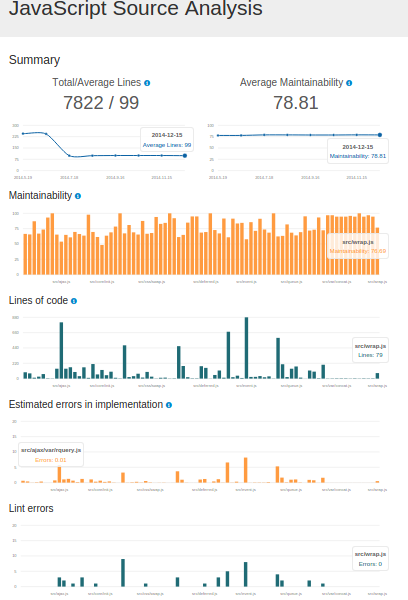
\includegraphics[width=\textwidth]{images/plato.png}
  \captionof{figure}{Javascript Source Analisis}
  \label{gfx/image}
\end{minipage}
\end{fixpic}
		
	\section{Processo di supporto}
		\subsection{Documentazione}
		
			\subsubsection{Scopo del processo}
			Questo processo ha lo scopo di definire degli strumenti per rendere coerente e uniforme l'insieme della documentazione prodotta nel ciclo di vita del software.
			
			\subsubsection{Procedure}
			Di seguito verranno presentate le regole e procedure che ogni componente di \textbf{\emph{Team404}} dovrà seguire nella redazione e la manutenzione  della documentazione di progetto. Il team ha scelto il linguaggio di markup \textbf{\LaTeX} per la  stesura dei suoi documenti per vari motivi:
			\begin{itemize}
			\item Permette una facile gestione degli indici e dei glossari.
			\item Dispone di  un sistema di "impaginazione" di alta resa tipografica.
			\item Permette di personalizzare comandi da usare in seguito.
			\item Dispone di numerose librerie con nuovi comandi.
	\end{itemize}		 
			\subsubsection{Template}
			Sarà creato un file \textit{template.tex}  che servirà di struttura iniziale a tutti i documenti in modo da garantire uniformità tra di loro.
			\subsubsection{Struttura dei documenti}
			\subsubsubsection{Comandi personalizzati}
			All'interno del file \textit{'template.tex'} verranno creati alcuni comandi generici da usare in modo da mantenere la stessa formattazione, quali:
			\begin{itemize}
			\item \textbf{\textbackslash addglos:} per indicare che la parola è nel glossario aggiungendo una 'G' a pedice alla parola.
			\item \textbf{\textbackslash beginglos:} per iniziare una sezione di termini del glossario.			
			\item \textbf{\textbackslash beginregistro:} per inserire una riga nel registro delle modifiche.  
			\item \textbf{\textbackslash fineglos:} per chiudere una sezione di termini del glossario. 
			\item \textbf{\textbackslash fineregistro:} per chiudere la tabella del registro delle modifiche.
			\item \textbf{\textbackslash introtab:}  per inserire la tabella di informazioni sul documento.
			\item \textbf{\textbackslash itemglos:} per inserire un termine e la sua descrizione in una sezione del glossario.
			\item \textbf{\textbackslash rigaregistro:} per inserire una riga nel registro delle modifiche. Ammette 4 parametri elencati in sezione.
			\item \textbf{\textbackslash subsubsubsection:}  per rendere disponibile la possibilità di usare una sotto sezione di terza livello.
			%\item \textbf{\textbackslash } 
			\end{itemize}
			\subsubsubsection{Frontespizio}
				Nella prima pagina verrà inserito il frontespizio che sarà costruito nel secondo ordine: 
				\begin{enumerate}
					\item \textbf{ Nome del progetto:} centrato e con una dimensione pari a 32 pt; 
					\item \textbf{ Logo del Gruppo:}  Il logo del gruppo è nel file "team\_not\_found.jpg" che si trova nella cartella principale dei documenti.
					\item \textbf{ Indirizzo email:} centrato e con una dimensione pari a 16 pt;
					\item \textbf{ Nome del documento:} centrato, in maiuscoletto, corredato dalla versione e con una dimensione pari a 24 pt; 
					\item \textbf{ Una tabella con informazioni generali del documento: }
					\begin{itemize}
						\item Nome del documento;
						\item Versione del documento;
						\item Data di redazione: deve essere indicata secondo il formato [ISO 8601];
						\item Redazione: elenco in ordine alfabetico dei redattori del documento;
						\item Verifica: elenco in ordine alfabetico dei Verificatori del documento;
						\item Approvazione: viene indicato il soggetto responsabile di aver approvato il documento;
						\item Uso: interno o esterno;
						\item Distribuzione: elenco in ordine alfabetico dei soggetti a cui verrà distribuito il documento in oggetto. 
					\end{itemize}
					\item \textbf{ Sommario:} brevissimo riassunto indicante lo scopo del documento.
				\end{enumerate}
				\subsubsubsection{Registro delle modifiche}
				Nella pagina successiva al frontespizio va inserito il registro delle modifiche per tener traccia di tutte le modifiche che verranno introdotte nel documento. Questo verrà fatto con una tabella formata come segue:
				\begin{itemize}
					\item \textbf{Versione:} la versione del documento dopo la modifica;
					\item \textbf{Autore:} l'autore della modifica con il ruolo tra parentesi;
					%\item \textbf{Ruolo:} il ruolo dell'autore nel gruppo;
					\item \textbf{Data:} la data della modifica;
					\item \textbf{Descrizione:} una breve indicazione della modifica effettuata.
				\end{itemize}
				\subsubsubsection{Indice}
				Per agevolare la consultazione e permettere una lettura ipertestuale e non necessariamente sequenziale, verrà creato una tabella dei contenuti in modo da facilitare la navigazione all'interno del documento.
				
				\subsubsubsection{Intestazione}
				Ogni pagina del documento ad eccezione della prima avrà un intestazione formata nel modo seguente:
				\begin{itemize}
				\item Logo del  gruppo a sinistra;
				\item Nome del progetto affianco al logo;
				\item Numero e titolo della sezione corrente a destra.
	\end{itemize}			
				\subsubsubsection{Piè di pagina}
				 Come per l'intestazione ogni pagina ad eccezione della prima avrà un piè di pagina formato nel modo seguente:
				 \begin{itemize}
				 \item L'e-mail del gruppo a sinistra;
				 \item Numero progressivo di pagina a destra.
	\end{itemize}			  
			\subsubsection{Versionamento}
			Ogni documento prodotto deve essere versionato in modo che chiunque lo utilizzi possa avere una cronologia delle sue modifiche. Ad ogni versione corrisponde una riga nel registro delle modifiche. Per numerare le versioni verrà adottata a la forma: \\ 
			 \textbf{{\centering  v.X.Y.Z }}
			\\
			dove \textbf{Z}:
			\begin{itemize}
			\item Parte da 0 e non è limitato superiormente;
			\item Viene incrementata ad ogni modifica del documento.
			\end{itemize}
			dove \textbf{Y}:
			\begin{itemize}
			\item Parte da 0 e non è limitato superiormente;
			\item Viene incrementato dal verificatore ad ogni verifica;
			\item Quando viene incrementato, \textbf{Z} viene azzerato.
			\end{itemize}
			dove \textbf{X}:
			\begin{itemize}
			\item Parte da 1 ed è limitato superiormente dal numero di revisioni;
			\item Viene incrementato dal Responsabile del gruppo quando approva il documento;
			\item Quanto viene incrementato, \textbf{Y} e \textbf{Z} vengono azzerati.
			\end{itemize}
			
			\subsubsection{Norme tipografiche}
				\subsubsubsection{Formattazione del testo}
				\begin{itemize}
				\item \textbf{Grassetto:} da usare per i titoli, per gli elementi di un elenco. Verrà usato anche per le parole significative;
				\item \textbf{Glossario:} viene aggiunta una lettera '\textbf{G}' a pedice a tutte le parole che hanno una corrispondenza nel glossario;
				\end{itemize}
				\subsubsubsection{Punteggiatura}
				\begin{itemize}
				\item \textbf{Maiuscolo:} la lettera iniziale maiuscola va utilizzata solo per i nomi propri o dopo i segni di punteggiatura punto, punto interrogativo e punto esclamativo;
				\item \textbf{Numeri:} per rappresentare i numeri verrà usato lo standard del sistema internazionale SI/ISO 31 che usa lo spazio come separatore delle migliaia e la virgola come separatore decimale (ad esempio 1 234 567,89); 
				\end{itemize}
				\subsubsubsection{Composizione del testo}
				\begin{itemize}
				\item \textbf{Elenco puntato:}
					\begin{itemize}
					\item[-] La prima parola va sempre con la lettera maiuscola;
					\item[-] La prima parola va in grassetto se è seguita da una descrizione della parola stessa;
					\item[-] Ogni punto dell'elenco deve terminare con un punto e virgola, tranne l'ultimo che deve terminare con un punto.
					\end{itemize}
				\end{itemize}
					
			\subsubsubsection{Formati}
			\begin{itemize}
				\item \textbf{Orario}: sarà usato lo standard ISO 8601 per rappresentare l'orario nel formato HH:MM dove:
					\begin{itemize}
					\item[-]HH: indica le ore, da scrivere sempre con 2 cifre;
					\item[-]MM: indica le minuti, da scrivere sempre con 2 cifre.
					\end{itemize}
				\item \textbf{Data:}  per agevolare la leggibilità, per la data verrà usato il formatto GG/MM/AAAA inverso allo standard dove:
				\begin{itemize}
				\item[-]GG: indica il giorno;
				\item[-]MM: indica il mese;
				\item[-]AAAA: indica l'anno.
				\end{itemize}
				\item \textbf{Link:} i link ipertestuali dovranno essere di colore blu.
			\end{itemize}
			\subsubsection{Componenti grafiche}
			\subsubsubsection{Tabelle}
				Ogni tabella nei documenti dovrà avere sotto di essa un numero identificativo e una didascalia. Inoltre alla fine di ogni documento dovrà apparire un elenco delle tabelle inserite.
				\subsubsubsection{Immagini}
					Le immagini da inserire in un documento dovranno essere raggruppate in una sotto cartella della cartella contenente il documento stesso; devono essere ben distanziate dai paragrafi che la precedono e da quelli che la seguono ed essere centrate orizzontalmente \\ \\ 
					 Inoltre alla fine di ogni documenti dovrà figurare un elenco delle figure e delle immagini presenti nel documento.
					 
			\subsubsection{Strumenti per la documentazione}
				
			\subsection{Verifica}
				\subsubsection{Scopo del processo}
					Questo processo ha per scopo di confermare che ogni componente software sviluppato sia conforme ai requisiti.		
				\subsubsection{Risultati osservabili}
				Il processo di verifica produce i seguenti risultati:
				\begin{itemize}
					\item l'individuazione e l'applicazione di una strategia di verifica;
					\item i criteri per la verifica di quanto prodotto dal software sono identificati;
					\item le attività di verifica sono state svolte;
					\item i difetti sono stati individuati e catalogati;
					\item i risultati della verifica sono resi disponibili ai proponenti.
				\end{itemize}
				
				\subsubsection{Tecniche di analisi}
				\subsubsubsection{Analisi statica}
				Tale tecnica è attuabile sia alla documentazione sia al codice, consiste nell'individuazione di errori ed anomalie ad esempio effettuando una lettura critica del testo a largo spettro oppure più mirata. Il Verificatore controllerà i documenti e il codice utilizzando le seguenti tecniche:
				\begin{itemize}
				\item[-]\textbf{Walkthrough\addglos:} Consiste in una lettura del documento/codice cercando errori ed anomalie a largo spettro senza un’idea precisa di quali tipi errori sarà possibile trovare. Ogni difetto rilevato sarà discusso con gli autori allo scopo di evitare incomprensioni e concordare sulle modifiche necessarie. L'utilizzo è previsto principalmente durante lo sviluppo iniziale, quando non si possiede ancora una chiara visione sui possibili errori. Un uso ripetuto di questa tecnica rende possibile la stesura di una lista di controlla. 		
				
				\item[-]\textbf{Inspection\addglos:} si basa sulla lettura mirata dei documenti/codice. Durante tale lettura si cercano gli errori segnalati nella lista di controllo. Progressivamente, con l'acquisizione di esperienza e grazie al precedente uso della tecnica di walkthrough\addglos, la lista di controllo viene estesa e specializzata, rendendo l'inspection\addglos sempre più efficace;
				\end{itemize}
				
				\subsubsubsection{Analisi dinamica}
				L'analisi dinamica si applica solamente al prodotto software e viene svolta durante l'esecuzione del codice mediante l'uso di appositi test per verificarne il funzionamento e rilevare possibili difetti d'implementazione. Affinché i test siano utili, devono essere ripetibili e devono trovare errori: infatti ogni test ha un costo, e un test che non aiuti a trovare dei difetti non ha motivo di esistere. I test sono ripetibili se, dati gli stessi dati in input, lo stesso ordine di esecuzione, lo stesso hardware e lo stesso software, ottengo in uscita gli stessi risultati;
				
				\subsubsection{Test}
								
				\subsubsubsection{Test di unità}
				Il test di unità verifica che ogni singola unità di prodotto software funzioni correttamente.
Attraverso questo test si verifica la correttezza di tutti i moduli base che compongono i software andando
a limitare gli errori di implementazione.
				\subsubsubsection{Test di integrazione}
				Il test di integrazione verifica che due o più moduli precedentemente verificati (con test di unità), una volta assemblati, funzionino ed interagiscano come previsto. Aiuta inoltre a rilevare eventuali difetti residui dei moduli, non individuati nella precedente fase di test. Questo test verifica inoltre l'interazione dei moduli prodotti con componenti software esterne come framework\addglos o librerie. È inoltre possibile che siano utilizzate delle componenti fittizie (driver\addglos e stub\addglos), impiegate al posto di determinati moduli (già pronti o ancora in costruzione) che abbiano un comportamento "sempre corretto" rispetto al contratto dei moduli che sostituiscono: questo permette di effettuare test sul corretto funzionamento dell'intero sottosistema e delle singole parti sviluppate.
				\subsubsubsection{Test di sistema}
				I test di sistema consistono nella validazione dei prodotti software. Questo test viene eseguito quando si ritiene il prodotto giunto ad una versione definitiva. Viene quindi verificata la completa copertura dei requisiti da parte del prodotto.
				\subsubsubsection{Test di regressione}
				Questo test viene eseguito subito dopo che una componente viene modificata. Consiste nel rieseguire tutti i test per verificare che dopo le modifiche il resto dei moduli continuino a funzionare in modo corretto. Il tracciamento aiuta a capire quali sono i test da ripetere (di ogni tipo) poiché potenzialmente a rischio in caso di modifica.
				\subsubsubsection{Test di accettazione}
				Coincide con il collaudo del software in presenza del proponente. Se tale test ha esito positivo, il prodotto sarà considerato sufficientemente maturo da permetterne il rilascio.
		\pagebreak
	\section{Processo Organizzativo}
		\subsection{Scopo del processo}
		Questo processo a come scopo di strutturare e facilitare l'organizzazione interna del gruppo stabilendo norme e modalità di comunicazione e di interazione.
		
		
		\subsection{Ruoli di progetto}
				\subsubsection{Definizione dei ruoli}
		Durante lo sviluppo di questo progetto vi sono diversi ruoli che  definiscono le responsabilità e i compiti da effettuare. Ogni membro del gruppo è tenuto a ricoprire tutti i ruoli almeno una volta. Vediamo nel dettaglio i vari ruoli:
		
		\subsubsubsection{Responsabile: }È il responsabile ultimo, per conto del suo gruppo, dei risultati del progetto.
Elabora ed emana piani e scadenze, ed approva l'emissione di documenti. 
Coordina le attività del gruppo, relazionandosi con il controllo di qualità interno al progetto. 
Redige Organigramma e Piano di Progetto, ed approva inoltre l'Offerta ed i relativi allegati.
			\subsubsubsection{Amministratore: }È responsabile dell'efficienza e dell'operatività dell'ambiente di sviluppo, della redazione e attuazione di piani e procedure di gestione per la qualità.
Controlla versioni e configurazioni del prodotto e gestisce l'archivio della documentazione di progetto. 
Collabora alla redazione del Piano di Progetto e nel contempo redige le Norme di Progetto per conto del Responsabile.
			\subsubsubsection{Analista: }È responsabile delle attività di analisi. 
Redige lo Studio di Fattibilità (documento interno al gruppo) e l'Analisi dei Requisiti.
			\subsubsubsection{Progettista: }È responsabile delle attività di progettazione. 
Redige Specifica Tecnica, Definizione di Prodotto e la parte programmatica del Piano di Qualifica.
			\subsubsubsection{Programmatore: }È responsabile delle attività di codifica miranti alla realizzazione del prodotto e delle componenti di ausilio necessarie per l'esecuzione delle prove di verifica e validazione.
			\subsubsubsection{Verificatore: }È responsabile delle attività di verifica.
Redige la parte retrospettiva del Piano di Qualifica che illustra l'esito e la completezza delle verifiche e delle prove effettuate secondo il piano.
		
				
		
		\subsection{Comunicazione}
			\subsubsection{Interna}			
			Per le comunicazioni ad uso interno del gruppo è stato creato un gruppo sull'App\addglos mobile "Whatsapp" per una rapida interazione tra i membri. Inoltre verrà usato il web tool Trello \addglos, il cui uso è spiegato nella sezione \ref{subsec:ticketing}.
			\subsubsection{Esterna}
			Il Responsabile di progetto sarà l'unico che potrà mantenere i contatti con individui esterni al gruppo, per farlo è stata creata una casella di posta elettronica: \url{team404swe@gmail.com}. Tutte le comunicazioni con il committente\addglos dovranno essere effettuate con questo indirizzo e-mail. Sarà suo dovere informare successivamente, gli altri componenti del gruppo di tutte le informazioni scambiate con il committente.
		\subsection{Incontri}
		\subsubsection{Interni}
		In caso di necessità, uno o più componenti del gruppo possono fare richiesta di una riunione al responsabile del progetto. Sarà compito di quest'ultimo autorizzarla o meno. 
		\subsubsection{Esterni}
		Sarà compito del Responsabile di progetto fissare incontri con il proponente\addglos o committenti\addglos e informare tutti i componenti del gruppo. Ogni riunione comprenderà la stesura di un verbale ufficiale contenete le seguenti informazioni:
\begin{itemize}
\item Data e ora;
\item Luogo;
\item Partecipanti esterni;
\item Partecipanti interni;
\item Domande e risposte.
\end{itemize}
		
		\subsection{Ticketing}
		\label{subsec:ticketing}
		Per gestire i compiti all'interno del gruppo è stato scelto il tool\addglos di gestione di progetti online Trello\addglos con il quale è possibile creare, assegnare, seguire e commentare delle liste composte da uno o più task\addglos personalizzabili. 
		\subsubsection{Struttura del ticket}
		Usando Trello\addglos ogni task\addglos  avrà le seguenti caratteristiche:
		
		\begin{enumerate}
		\item \textbf{Titolo:} riassume in modo conciso il task\addglos;
		\item \textbf{Membri:} sono i membri ai quali viene assegnato il task;
		\item \textbf{Label:} identifica il tipo di task\addglos e gli assegna un colore;
		\item \textbf{Data di scadenza:} indica la data entro la quale il task deve essere completato;
		\item \textbf{Descrizione:} è una descrizione più ampia che può essere inserita per spiegare il compito da svolgere;
		\item \textbf{Allegato:} permette di allegare un file al task;
		\item \textbf{Stato:} rappresenta lo stato del task che può essere successivamente 'Accettato', 'Eseguito' e poi 'Verificato' ed include anche una barra di progressione da 0 a 100\%; 
		\item \textbf{Commenti:} è una funzionalità che permette ai membri di scambiare parere e informazioni riguardanti il task.
		
		\end{enumerate}
		
		% da sistemare perché 
		\begin{figure}[htbp]
		\centering
		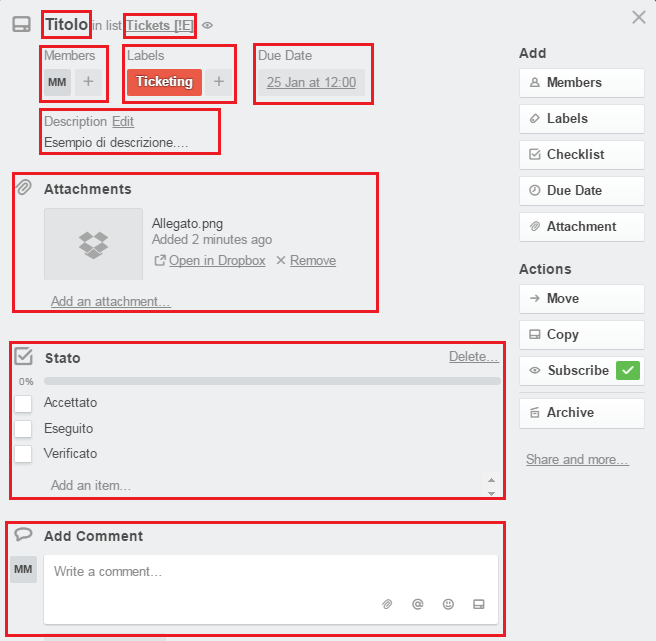
\includegraphics[scale=0.50]{./images/tuto2.png}
		\caption{Esempio di configurazione di un task su Trello}			
			
		\end{figure}
		
		
		
		\subsection{Strumenti di progetto} \label{s:strum} 	
	
		\subsubsection{Sistema operativo}
		La scelta del sistema operativo da utilizzare sarà a discrezione di ogni componente del gruppo, dato che non influirà sul funzionamento dell'applicazione.
		\subsubsection{Codifica dei caratteri}
		Per assicurarsi la corretta visualizzazione dei caratteri accentati tutti i file testuali presenti nel repository\addglos(sia codice sorgente che documentazione) devono essere memorizzati con la codifica\textbf{ UTF-8\addglos.}
		\subsubsection{Versionamento}
		Per il versionamento dei documenti e del codice viene usato \textbf{Git\addglos} (\url{http://git-scm.com/}). Si utilizzerà il servizio \textbf{GitHub\addglos} per creare e gestire i repository privati utilizzati dal gruppo.
			
	\subsection{Produzione dei documenti}
	
	\subsubsection{Dropbox}
	Per la condivisione di file e documenti non soggetti a controllo di versione tra i membri del gruppo. A questo scopo è stata creata una cartella che contiene anche i vari  manuali degli strumenti di interesse per il progetto.
	\subsubsection{Editor}
	Come editor per i documenti viene scelto TexMaker\addglos, un programma open source per scrivere documenti in \LaTeX  che offre multiple funzionalità quali il supporto dell'unicode, la colorazione sintattica e la correzione autografica nonché la possibilità di esportare il documento in HTML o in formato OpenDocument\addglos.
	\subsubsection{Correttore ortografico}
	Come correttore ortografico dei documenti prodotti verrà utilizzato il software \textbf{MySpell}\addglos integrato nell'editor TexMaker.
	\newpage
	
		
	\end{document}
